%!TEX root = ../thesis.tex
%*******************************************************************************
%****************************** Third Chapter **********************************
%*******************************************************************************

\chapter{Matherial and methods}
\label{chap:matherial_methods}
\ifpdf
    \graphicspath{{Chapter3/Figs/Raster/}{Chapter3/Figs/PDF/}{Chapter3/Figs/}}
\else
    \graphicspath{{Chapter3/Figs/Vector/}{Chapter3/Figs/}}
\fi


\section{Constitution du benchmark} % (fold)
\label{sec:constitution_du_benchmark}

\victor{données specifiquement utilisées}

\victor{simulateur rapide}

\section{Evaluation metric} % (fold)
\label{sec:evaluation_metric}

Many methods to estimate the parameter of interest and its variance are available.
If changing the set of hyper parameter for the learning procedure is considered as changing the method then countless methods are to be evaluated.
Automating the measure of the performances of a proposed method is crucial to select the best method.
In this section is described a simple but general procedure to measure the performances of a given method.

The usual criterions to evaluate an estimator $\htheta$ are the bias, the variance and the mean squared error defined as follow :
\begin{equation}
  Bias(\htheta) = \EE[\htheta] - \thetas
\end{equation}
\begin{equation}
  Var(\htheta) = \EE[ (\htheta - \EE[\htheta])^2 ] = \EE[\htheta^2] - (\EE[\htheta])^2
\end{equation}
\begin{equation}
  MSE(\htheta) = \EE[(\htheta - \thetas)^2] = Var(\htheta) + [Bias(\htheta)]^2
\end{equation}

To evaluate these criterion we need to repeat the experiement $N$ times leading to many estimation of the parameters $\hmu^{(k)}$ and $\hshmu^{(k)}$.
Repeating the experiment can be done through cross-validation methods.


\subsection{Evaluation of the parameter of interest estimator} % (fold)
\label{sub:evaluation_of_the_parameter_of_interest_estimator}

First, let's focus on evaluating the estimator of the parameter of insterest $\hmu$.
The true value of $\mu$, noted $\mus$, is available during tests since it is an input of the simulator.

From the estimation of its expected value
\begin{equation}
  \EE[\hmu] \approx <\hmu^{(k)}>_k = \frac{1}{N} \sum_{k} \hmu^{(k)}
\end{equation}
it is possible to estimated the criterions

\begin{equation}
  Bias(\hmu) \approx <\hmu^{(k)}>_k - \mus
\end{equation}
\begin{equation}
  \label{eq:var_hmu}
  Var(\hmu) \approx <\hmu^{(k)} \times \hmu^{(k)}>_k - (<\hmu^{(k)}>_k)^2
\end{equation}
\begin{equation}
  MSE(\hmu) = Var(\hmu) + [Bias(\hmu)]^2
\end{equation}

\subsection{Evaluation of the variance estimator} % (fold)
\label{sub:evaluation_of_the_variance_estimator}

The evaluation of the variance estimator $\hshmu$ could be done in the same way if the true variance $Var(\hmu)$ can be computed.
If this is not the case an approximation is available using \autoref{eq:var_hmu}.

\begin{equation}
  Bias(\hshmu) \approx <\hshmu^{(k)}>_k - Var(\hmu)
\end{equation}
\begin{equation}
  Var(\hshmu) \approx <\hshmu^{(k)} \times \hshmu^{(k)}>_k - (<\hshmu^{(k)}>_k)^2
\end{equation}
\begin{equation}
  MSE(\hmu) = Var(\hshmu) + [Bias(\hshmu)]^2
\end{equation}



\section{"Domain adaptation"} % (fold)
\label{sec:domain_adaptation}

\victor{Tangent prop}

Tangent Propagation is learning to become robust to a known geometrical/differentiable transformation of the input features.

\victor{how Pivot is "domain adaptation"}

Pivot network are trained to become robust to the variation of a known feature (which may not be an input feature).


\section{More direct approach} % (fold)
\label{sec:more_direct_approach}

\victor{INFERNO}

\victor{Regression}

\victor{Montrer sur des toys}

\victor{VAE}




\begin{figure}[htb]
  \centering
  \begin{subfigure}[t]{0.49\linewidth}
    
\includegraphics[width=\linewidth]{minion}
    \caption{Minions}
    \label{fig:minion}
  \end{subfigure}%
  \hfill
  \begin{subfigure}[t]{0.49\linewidth}
    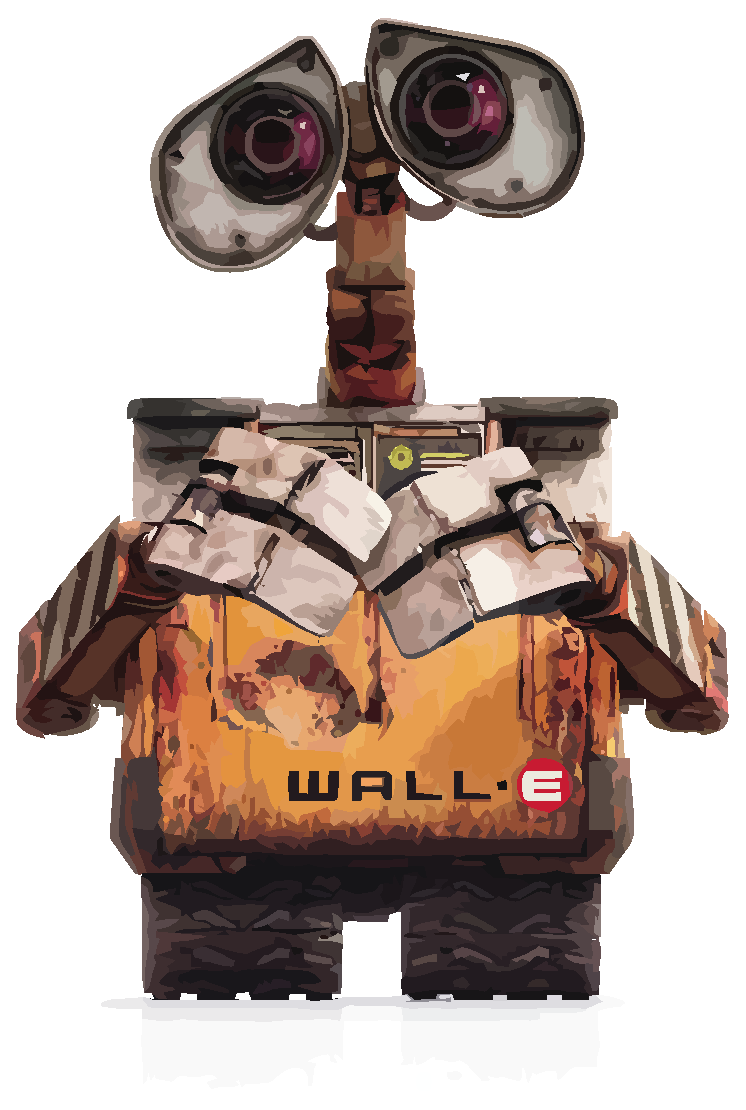
\includegraphics[width=\linewidth]{WallE}
    \caption{"Eve"}
    \label{fig:walle}
  \end{subfigure}
  \caption{Comparison Minions (left) and WallE (right)}
  \label{fig:comparision}
\end{figure}
